%!TEX root = ../Thesis.tex
\chapter{Discussion and conclusion}

In agreement with Novo Nordisk, the specific methods of combining permeability predictions and solubility predictions and the actual suggested candidates have not been included in this thesis. However the distribution of solubility predictions and permeation predictions is a good basis for a discussion of whether it is possible to search for permeation enhancers that are both soluble and sufficiently potent.

\subsection{Is predicted potency the same as insolubility}
In Figure \ref{predictionsCombined} the predicted solubility and permeability are plotted for 10,000 molecules. Permeability predictions are based on a model similar to the one described in article of Section \ref{article:predAbs}. As the predictive model rely on molecular descriptor computations with the MOE software suite, and this take in average 1 second per molecule to compute. The full available million molecule search set would have taken 11 days to run. To narrow down the search set, molecules were selected by criteria of rotatable bonds and molar weight in anticipation, that molecules with less than a certain fraction of rotatable bonds would likely not have fatty carbon chains.

As discussed in Section \ref{predPerm:workflow}, it was a major consideration, that the permeability model and solubility model both perhaps only would recognize lipophilicity-like properties as predictors, and thus perform exactly opposite predictions. However this seems not to be the case for the 10,000 predicted molecules, as there are molecules with various predicted ratios between solubility and permeability enhancement. However, in the Figure no molecules ocour in the top right 'unrealistic' corner, where molecules would be predicted as both very soluble and very potent.

\begin{figure}[!htbp]
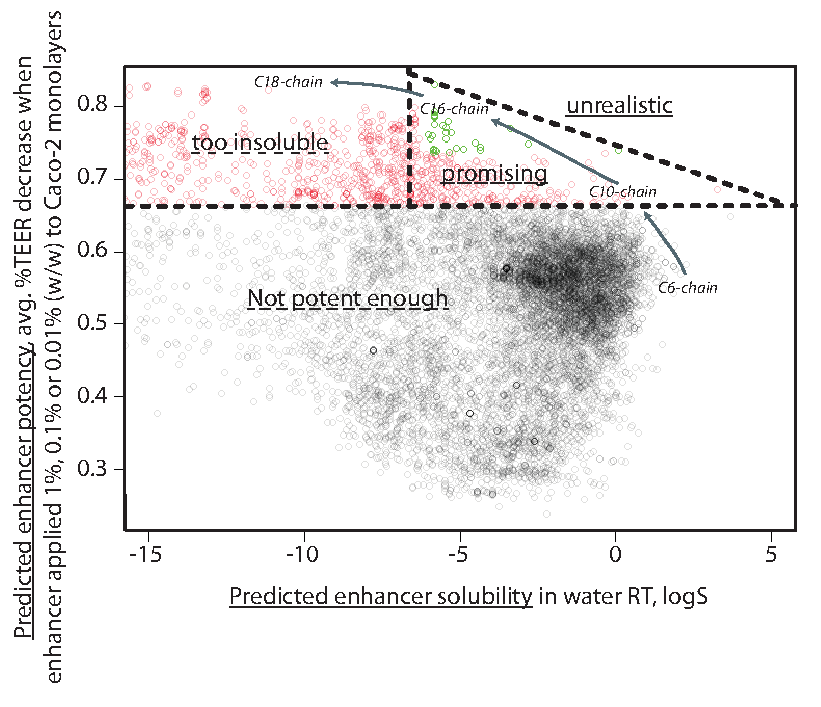
\includegraphics[width=\textwidth,height=\textheight,keepaspectratio]{graphics/screened_molecules3.pdf}
\caption{Predictions of logS water solubility and permeation enhancement in Caco-2 model for 10,000 compounds. Few molecules are both soluble and potent permeation enhancers. Figure has been segmented into groups of 'too insoluble', 'not potent enough', 'promising' and 'unrealistic'. For a given group of surfactant permeation enhancers, the carbon chain can be reduced or elongated. The arrows from C6 to C18 exemplify a given enhancer group, where the C18 is too insolble and C6 not potent enough. For a given other enhancer family with less favorable head group may not cross into the 'promising' segment for any carbon chain length.}
\label{predictionsCombined}
\end{figure}

In Figure \ref{predictionsCombined} the majority of molecules are not potent enough. Sodium caprate has been set as the lower bar of required potency = 0.67. A potency of 0.67 predicts that if a compound was used as permation enhancer and added to three Caco-2 monolayers in solution at 1\%, 0.1\% and 0.01\% \textit{(w/w)}, the electrical resistance across the monolayers would in average be lowered 67\%. As discussed in article from Section \ref{article:predAbs}, the permeation model overestimate the potency of non permeation enhancers, as the training set contained no non-permation enhancers. Thus the permeation model likely has not learned to separate non potent from weekly potent. However, a permeation enhancement potency below carbon chain C10 is probably too weak, since no C8 or C6 permation enhancers have been successfully included in a formulation. Therefore the most important task of the model is to distinguish the highly potent enhancers from the medium potent.

\subsection{Uncertainty of predictions}
In Section \ref{article:predAbs} the root mean square prediction error of the permeation enhancer model was found to be 0.16, on the defined potency scale from 0 to 1. The prediction error was estimated by cross-validation and on a external data set. Therefore it is reasonable to expect the model can recognize molecules as highly potent, medium potent or non-potent permeation enhancers. The prediction error (standard deviation) of the solubility model as discussed in the results part of the draft "Learning the structure of random forest models QSAR modelling: Predicting molecular Solubilty" in Section \ref{article:solubility} estimated by cross-validation is 0.64 on the logS scale. A standard deviation on logS scale of 0.64 translates to a 4-fold deviation in absolute solubility. As the training molecules in the \textit{Huskonnen et al} data set \cite{palmer2007random} span the logS scale from -10 to +2, a prediction error of 0.64(RMSE) seems as a quite accurate model. Likewise, the cross-validated estimated explained variance of the model is 90\%. However to function as an permeation enhancer, if logS is below -6, the dissolution rate would likely be too slow.

Most surfactant based permeation enhancers have an ability to form micelles, such that the apparent solubility of very lipophilic permeation enhancers could be close -1. However the lipophilic permeation enhancers will have a low dissolution rate. The predictions of a theoretical logS replaces the intrinsic dissolution rate, that likely would have been the best property to predict. No large public data set, was found for intrinsic dissolution

Solubility models \cite{delaney2004esol,palmer2007random} are mainly derived from solubility measurements at room temperature 20-25 degrees Celcius. As the solubilization occurs at 37 degrees Celcius, some molecules may improve solubility more than others. Noyes-Whitney dissolution rate equation predict dissolution as proportional to the concentration gradient. The more soluble an enhancer is, the proportionally faster it can ideally pass from solid form to mono-meric form and diffuse away from the tablet. The temperature sensitivity of molecules has not been accounted for. All logS prediction match 20 to 25 degrees celcius. Most likely the majority of molecules will have a higher logS value at 37 degrees, however some molecules may be more sensitive to temperature than others. This will contribute with extra uncertainty, when extrapolating to 37 degrees Celcius. One future approach could be to model the temperature sensitivity for a smaller data set and use these temperature sensitivity predictions to correct predictions at room temperature \cite{klimenko2016novel}.


\subsection{Interplay of dissolution rate and insulin permeability}
Permeation enhancers can increase the permeability of insulin across the epithelial barrier. Insulin degrade with time due to enzymes in the luminal space of the small intestine. To reduce the time in luminal space, the permeation enhancer must contribute to a fast efficient dissolution of the tablet. A very slow release will give apparent zero-order enzyme reactions an advantage to break down all insulin. Also the permeation enhancer may be cleared from the site of action faster than the release from the tablet, such that the overall concentration of permeation enhancer in the epithelial membrane will be too low to have an effect.

\begin{figure}[!htpb]
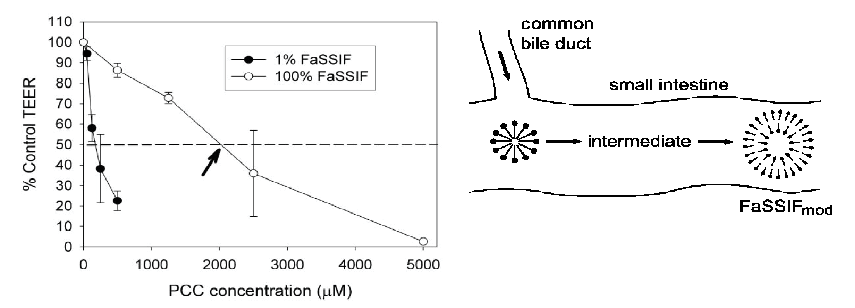
\includegraphics[width=\textwidth,height=\textheight,keepaspectratio]{graphics/develop_fassif.pdf}
\caption{Two figures copied from \cite{tippin2008biorelevant,nawroth2011liposome} to illustrate why the potency of lipophilic permeation enhancers are likely overestimated in \textit{in-vitro} studies using surfactant free buffers. Left, palmitoyl carnitine a C16 surfactant enhancer was found by Tippin \textit{et al} to be 12 times less potent in a FaSSIF buffer with taurocholate and lechitine an EC$_{50}$. Right, in the intestinal lumen taurocholate and lechitine will be released from the bile duct and form micelles and liposomes. Small concentrations of long chain lipophilic enhancer will absorbed by the liposomes instead of the epithelial membrane.S}
\label{devel_fassif}
\end{figure}

Identifying new potent enhancers with the Caco-2 cell model do not emphasize the dissolution speed. As a substitute for intrinsic dissolution speed measurements, logS-solubility was used instead, as intrinsic dissolution measurements were too sparse and not available in the public domain. Predicting both solubility and permeation enhancement allowed to correct for the over-optimistic scoring of lipophilic permeation enhancers in the caco-2 model. As the Caco-2 model uses watery HBSS buffer, the lipophilic permeation enhancers will have no other place to bind than the epithelial membrane. However under \textit{in-vivo} conditions, there will be plenty of competing sites to bind such as billary liposomes and micelles. Tippin \textit{et al} has showed that in-vitro models using HBSS buffers favor lipophilic permeation enhancers \cite{tippin2008biorelevant}. In a buffer such as FaSSIF, that contain small amounts of inert surfactants, the lipophilic enhancers will be absorbed into the inert micelles instead of the site of action. On the other hand, a medium potent permeation enhancer such as sodium caprate can dissolve from the tablet fast enough, that the concentration of caprate is much higher than the inert surfactants. The change of potency for a lipophilic enhancer palmitoyl carnitine is described in Figure \ref{devel_fassif}.


\subsection{Interpretation of random forest}
The regression random forest learner was used to build predictive models. The explicit structure of the trained random forest models is too complicated to comprehend. Feature contributions was used, in order to evaluate what properties of molecules that constitutes soluble and potent permeation enhancers. With forest floor plots a distinct interaction in the trained random forest model structure was discovered. Specifically it was recognized that long carbon chains only increased the predicted potency, if the molecule also had a dipole moment above a certain threshold. This seems to be a reasonable rule to identify surfactants, as these must have both a hydrophile and lipophile domain and there will likely be a dipole moment between the two domains \cite{rosen2012surfactants}.

As the forest floor method of visualizing feature contributions, had not been described before in literature and it seemed to have some advantages over other diagnostic methods for similar purposes, it was very interesting to develop a generic visualization tool which could assist other random forest users in various fields to understand the overall structure of the trained model. The outcome has been a statistical package computing feature contributions and diagnostic tools to direct how the high dimensional model can be reduced to low dimensional visualizations. Today the package has been downloaded 5000 times, I hope to see the amount of users grow substantially the next years.